\documentclass{article}

\usepackage{fullpage}
\usepackage{color}
\usepackage{amsmath}
\usepackage{url}
\usepackage{verbatim}
\usepackage{graphicx}
\usepackage{parskip}
\usepackage{amssymb}
\usepackage{nicefrac}
\usepackage{listings} 
\usepackage{algorithm2e}

\def\rubric#1{\gre{Rubric: \{#1\}}}{}

% Colors
\definecolor{blu}{rgb}{0,0,1}
\def\blu#1{{\color{blu}#1}}
\definecolor{gre}{rgb}{0,.5,0}
\def\gre#1{{\color{gre}#1}}
\definecolor{red}{rgb}{1,0,0}
\def\red#1{{\color{red}#1}}
\def\norm#1{\|#1\|}

% Math
\def\R{\mathbb{R}}
\def\argmax{\mathop{\rm arg\,max}}
\def\argmin{\mathop{\rm arg\,min}}
\newcommand{\mat}[1]{\begin{bmatrix}#1\end{bmatrix}}
\newcommand{\alignStar}[1]{\begin{align*}#1\end{align*}}
\def\half{\frac 1 2}

% LaTeX
\newcommand{\fig}[2]{\includegraphics[width=#1\textwidth]{#2}}
\newcommand{\centerfig}[2]{\begin{center}\includegraphics[width=#1\textwidth]{#2}\end{center}}
\newcommand{\matCode}[1]{\lstinputlisting[language=Matlab]{a2f/#1.m}}
\def\items#1{\begin{itemize}#1\end{itemize}}
\def\enum#1{\begin{enumerate}#1\end{enumerate}}

\begin{document}

\section{Vectors, Matrices, and Quadratic Functions}

\subsection{Basic Operations}
\rubric{reasoning:3}

\noindent Using the definitions below,
\[
\alpha = 5,\quad
x = \left[\begin{array}{c}
2\\
-3\\
\end{array}\right], \quad
y = \left[\begin{array}{c}
1\\
4\\
\end{array}\right],\quad
z = \left[\begin{array}{c}
2\\
0\\
1\end{array}\right],
\quad
A = \left[\begin{array}{ccc}
1 & 2\\
2 & 3\\
3 & -2
\end{array}\right],
\]
\blu{evaluate the following expressions} (show your work, but you may use answers from previous parts to simplify calculations):\\

\enum{
\item $x^Tx$ =
$\begin{bmatrix}
  2  & {-3}
\end{bmatrix}$
$\begin{bmatrix}
  2 \\
  -3 \\
\end{bmatrix}$
= 
$\begin{bmatrix}
  13
\end{bmatrix}$
\item $\norm{x}^2$ 
=
$\begin{bmatrix}
	2 \\
	-3 \\  
\end{bmatrix}$
$\begin{bmatrix}
	2 \\
	-3 \\   
\end{bmatrix}$
=
$2^2 + (-3)^2$
=
13
\item $x^T(x + \alpha y)$
=
$\begin{bmatrix}
	2 & -3
\end{bmatrix}$
(
$\begin{bmatrix}
	2 \\
	-3 \\   
\end{bmatrix}$
+
$5\begin{bmatrix}
	1 \\
	4 \\   
\end{bmatrix}$
)
=
$\begin{bmatrix}
	2 & -3
\end{bmatrix}$
(
$\begin{bmatrix}
	2 \\
	-3 \\   
\end{bmatrix}$
+
$\begin{bmatrix}
	5 \\
	20 \\   
\end{bmatrix}$
)
=
$\begin{bmatrix}
	2 & -3   
\end{bmatrix}$
$\begin{bmatrix}
	7 \\
	17 \\   
\end{bmatrix}$
=
$(7 * 2) + (-3 * 17)$
=
$14 + (-51)$
=
$-37$
\item $Ax$
=
$\begin{bmatrix}
	1 & 2 \\
	2 & 3 \\
	3 & - 2 \\  
\end{bmatrix}$
$\begin{bmatrix}
	2 \\
	-3 \\   
\end{bmatrix}$
=
$\begin{bmatrix}
	-4 \\
	-5 \\
	12 \\   
\end{bmatrix}$
\item $z^TAx$
=
$\begin{bmatrix}
	2 & 0 & 1  
\end{bmatrix}$
$\begin{bmatrix}
	-4 \\
	-5 \\
	12 \\   
\end{bmatrix}$
=
$\begin{bmatrix}
	(-4 * 2) + 0 + (12)   
\end{bmatrix}$
=
$\begin{bmatrix}
	4   
\end{bmatrix}$
\item $A^TA$
=
$\begin{bmatrix}
	1 & 2 & 3 \\
	2 & 3 & -2 \\
\end{bmatrix}$
$\begin{bmatrix}
	1 & 2 \\
	2 & 3 \\
	3 & -2 \\  
\end{bmatrix}$
=
$\begin{bmatrix}
	14 & 2 \\
	2 & 17 \\   
\end{bmatrix}$
}

If $\{\alpha,\beta\}$ are scalars, $\{x,y,z\}$ are real-valued column-vectors of length $d$,
and $\{A,B,C\}$ are real-valued $d\times d$ matrices, \blu{state whether each of the below statements is true or false in general
and give a short explanation.}
\enum{
\addtocounter{enumi}{6}
\item $yy^Ty = \norm{y}^2y$. \\
Always true because $||y||^2 = y^Ty$ and is a scalar.
\item $x^TA^T(Ay + Az) = x^TA^TAy + z^TA^TAx$. \\
False / not always true because it is missing a term at the end.
\item $x^T(B + C) = Bx + Cx$. \\
False because $a^T(b +c) = a^Tb + a^Tc$ but $a^Tb = b^Ta$ (and either case would be false, actually.)
\item $(A + BC)^T = A^T + C^TB^T$.
True because $A^T + (BC)^T = A^T + C^TB^T$.
\item $(x-y)^T(x-y) = \norm{x}^2 - x^Ty + \norm{y}^2$.
False because when expanded out, it becomes: $||x||^2 - x^Ty - y^Tx + ||y||^2$. The middle term $-x^Ty - y^Tx$ does not equal $-x^Ty$, instead, it equals $2(-x^Ty)$.
\item $(x-y)^T(x+y) = \norm{x}^2 - \norm{y}^2$.
True because when expanded out, it becomes $||x||^2 + yx^T - y^Tx - ||y||^2$. As $yx^T = xy^T$, the middle term $xy^T - y^Tx$ cancels out.
}

Hint: check the dimensions of the result, and remember that matrix multiplication is generally not commutative.

\subsection{Converting to Matrix/Vector/Norm Notation}
\rubric{reasoning:2}

Using our standard supervised learning notation ($X$, $y$, $w$)
express the following functions in terms of vectors, matrices, and norms (there should be no summations or maximums).
{\enum{
\item $\sum_{i=1}^n |w^Tx_i - y_i|$ = 
$||Xw - Y||_1$
\item $\max_{i \in \{1,2,\dots,n\}} |w^Tx_i  - y_i| + \frac{\lambda}{2}\sum_{j=1}^d w_j^2$ =
$||Xw - Y||_\infty + \frac{\lambda}{2}||w||^2_2$
\item $\sum_{i=1}^n z_i (w^Tx_i - y_i)^2 + \lambda \sum_{j=1}^{d} |w_j|$ =
$$\sum_{i=1}^n z_i(w^Tx_i - y_i)^2 + \sum_{j=1}^d|w_j|$$
$$\sum(x_iw - y_i)z_i(x_iw - y_i) + x||w||_1$$
$$(Xw-y)^T\begin{bmatrix} z_1(Xw-y)_1 \\ \vdots \\ z_n(Xw-y)_n \end{bmatrix}$$
$$(Xw - Y)^TZ(Xw - Y) + \lambda||w||_1$$
}}

\subsection{Minimizing Quadratic Functions as Linear Systems}
\rubric{reasoning:3}

Write finding a minimizer $w$ of the functions below as a system of linear equations (using vector/matrix notation and simplifying as much as possible). Note that all the functions below are convex  so finding a $w$ with $\nabla f(w) = 0$ is sufficient to minimize the functions (but show your work in getting to this point).
{\enum{
\item $f(w) = \frac{1}{2}\norm{w-v}^2$
$$\nabla f(w) = 0$$
$$\nabla \frac{1}{2}(w-v)^T(w-v) = 0$$
$$\nabla w^Tw - v^Tw - w^Tv + v^Tv$$
$$\nabla w^Tw - 2v^Tw + v^Tv = 0$$
$$2w - 2v = 0$$
$$2w = 2v$$
$$w = v$$
\item $f(w) = \frac{1}{2}\norm{w}^2 + w^TX^Ty$
$$\nabla f(w) = 0$$
$$\frac{1}{2}(2w) + x^Ty = 0$$
$$w = x^Ty$$
\item $f(w) = \frac{1}{2}\sum_{i=1}^n z_i (w^Tx_i - y_i)^2$
$$\nabla f(w) = 0$$
$$f'(w) = \frac{1}{2}(2z_1x_1(w^Tx_1 - y_1) + 2z_2x_2(w^Tx_2 - y_2) + \ldots + 2z_nx_n(w^Tx_n - y_n)) = 0$$
$$w(z_1x_1^Tx_1 + z_2x_2^Tx_2 + \ldots + z_nx_n^Tx_n) - (z_1x_1y_1 + z_2x_2y_2 + \ldots + z_nx_ny_n) = 0$$
$$w(X^TZX) - X^T2Y = 0$$
$$w = (X^TZX)^{-1}X^TZY$$  
}}

\section{Robust Regression and Gradient Descent}

If you run \verb|python main.py -q 2|, it will load a one-dimensional regression
dataset that has a non-trivial number of `outlier' data points.
These points do not fit the general trend of the rest of the data,
and pull the least squares model away from the main downward trend that most data points exhibit:
\centerfig{.7}{../figs/least_squares_outliers.pdf}

Note: we are fitting the regression without an intercept here, just for simplicity of the homework question.
In reality one would rarely do this. But here it's OK because the ``true'' line 
passes through the origin (by design). In Q3.1 we'll address this explicitly.

\subsection{Weighted Least Squares in One Dimension}
\rubric{code:3}

One of the most common variations on least squares is \emph{weighted} least squares. In this formulation, we have a weight $z_i$ for every training example. To fit the model, we minimize the weighted squared error,
\[
f(w) =  \frac{1}{2}\sum_{i=1}^n z_i(w^Tx_i - y_i)^2.
\]
In this formulation, the model focuses on making the error small for examples $i$ where $z_i$ is high. Similarly, if $z_i$ is low then the model allows a larger error.

Complete the model class, \emph{WeightedLeastSquares}, that implements this model
(note that Q1.3.3 asks you to show how this formulation can be solved as a linear system).
Apply this model to the data containing outliers, setting $z = 1$ for the first
$400$ data points and $z = 0.1$ for the last $100$ data points (which are the outliers).
\blu{Hand in your code and the updated plot}.

Code can be found in $code/linear\_model.py$.
\\ 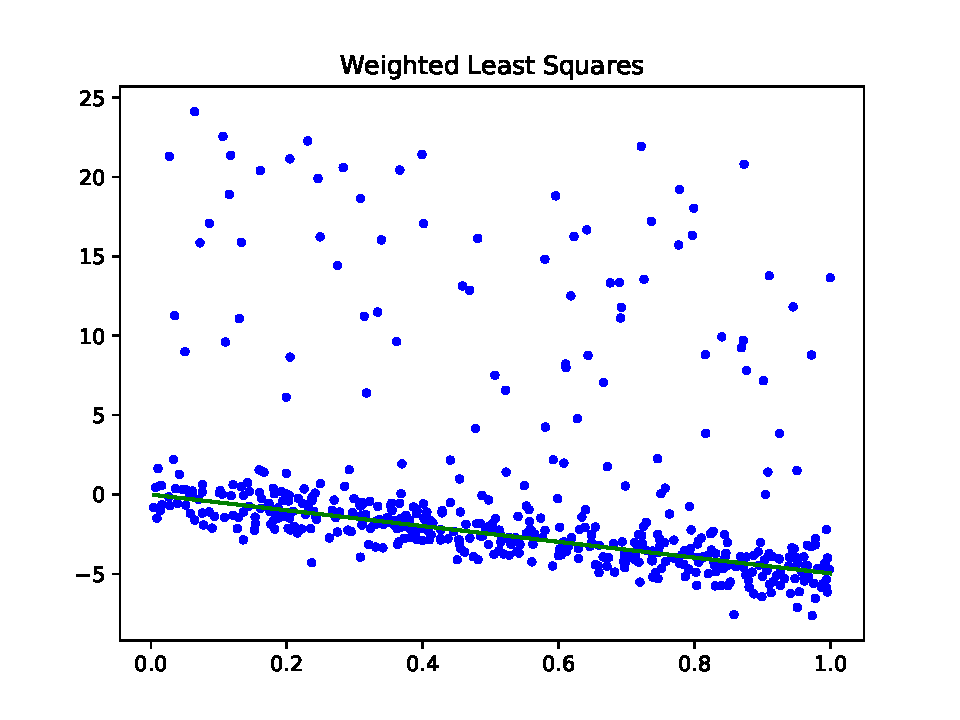
\includegraphics{../figs/least_squares_outliers_weighted.pdf}


\subsection{Smooth Approximation to the L1-Norm}
\rubric{reasoning:3}

Unfortunately, we typically do not know the identities of the outliers. In situations where we suspect that there are outliers, but we do not know which examples are outliers, it makes sense to use a loss function that is more robust to outliers. In class, we discussed using the sum of absolute values objective,
\[
f(w) = \sum_{i=1}^n |w^Tx_i - y_i|.
\]
This is less sensitive to outliers than least squares, but it is non-differentiable and harder to optimize. Nevertheless, there are various smooth approximations to the absolute value function that are easy to optimize. One possible approximation is to use the log-sum-exp approximation of the max function\footnote{Other possibilities are the Huber loss, or $|r|\approx \sqrt{r^2+\epsilon}$ for some small $\epsilon$.}:
\[
|r| = \max\{r, -r\} \approx \log(\exp(r) + \exp(-r)).
\]
Using this approximation, we obtain an objective of the form
\[
f(w) {=} \sum_{i=1}^n  \log\left(\exp(w^Tx_i - y_i) + \exp(y_i - w^Tx_i)\right).
\]
which is smooth but less sensitive to outliers than the squared error. \blu{Derive
 the gradient $\nabla f$ of this function with respect to $w$. You should show your work but you do \underline{not} have to express the final result in matrix notation.}

First, let $r$ be $(w^Tx_i - y_i)$. \\\\
To calculate the gradient of $f(w)$, we have to find the derivative of every $w_i$. We will begin by calculating the derivative of $w_1$ as an example.

$$f'(w_1) {=} \sum_{i=1}^n  \frac{d}{dw_1} \log\left(e^{r} + e^{-r}\right)$$
$$\sum_{i=1}^n (\frac{1}{e^r + e^{-r}})\frac{d}{dw_1}(e^r + e^{-r})$$
$$\sum_{i=1}^n  (\frac{1}{e^r + e^{-r}})(e^r\frac{d}{dw_1}r + e^{-r}\frac{d}{dw_1}{-r})$$
$$\frac{d}{dw_1}r = \frac{d}{dw_1}(w^Tx_i - y_i) = \frac{d}{dw_1}w_1x_{i1} + w_2x_{i2} + \ldots + w_nx_{in} = x_{i1}$$
$$\frac{d}{dw_1}{-r} = \frac{d}{dw_1}(y_i - w^Tx_i) = -x_{i1}$$
$$\sum_{i=1}^n  (\frac{1}{e^r + e^{-r}})(e^rx_{i1} + e^{-r}-x_{i1})$$
$$\nabla f(w) =
\begin{bmatrix}
	\sum_{i=1}^n  (\frac{1}{e^r + e^{-r}})(e^rx_{i1} + e^{-r}-x_{i1}) \\
	\sum_{i=1}^n  (\frac{1}{e^r + e^{-r}})(e^rx_{i2} + e^{-r}-x_{i2}) \\
	\vdots \\
	\sum_{i=1}^n  (\frac{1}{e^r + e^{-r}})(e^rx_{in} + e^{-r}-x_{in}) \\
\end{bmatrix}$$


\subsection{Robust Regression}
\rubric{code:2,reasoning:1}

The class \emph{LinearModelGradient} is the same as \emph{LeastSquares}, except that it fits the least squares model using a gradient descent method. If you run \verb|python main.py -q 2.3| you'll see it produces the same fit as we obtained using the normal equations.

The typical input to a gradient method is a function that, given $w$, returns $f(w)$ and $\nabla f(w)$. See \emph{funObj} in \emph{LinearModelGradient} for an example. Note that the \emph{fit} function of \emph{LinearModelGradient} also has a numerical check that the gradient code is approximately correct, since implementing gradients is often error-prone.\footnote{Sometimes the numerical gradient checker itself can be wrong. See CPSC 303 for a lot more on numerical differentiation.}

An advantage of gradient-based strategies is that they are able to solve
problems that do not have closed-form solutions, such as the formulation from the
previous section. The class \emph{LinearModelGradient} has most of the implementation
of a gradient-based strategy for fitting the robust regression model under the log-sum-exp approximation.
The only part missing is the function and gradient calculation inside the \emph{funObj} code.
\blu{Modify \emph{funObj} to implement the objective function and gradient based on the smooth
approximation to the absolute value function (from the previous section). Hand in your code, as well
as the plot obtained using this robust regression approach.}
\\
Code can be found in $code/linear\_model.py$.
\\ 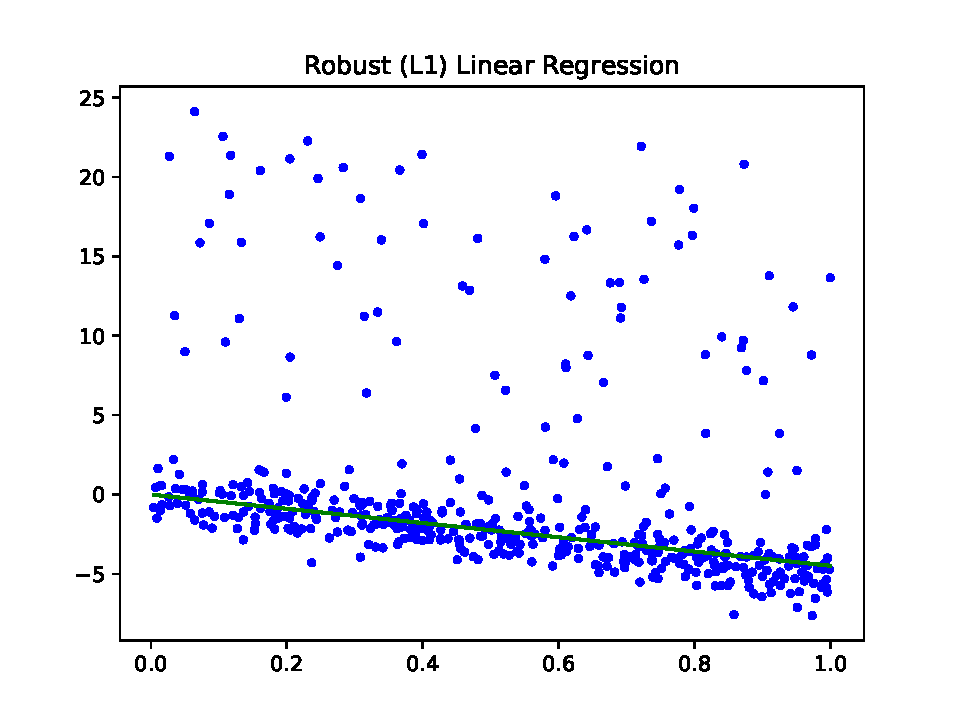
\includegraphics{../figs/least_squares_robust.pdf}


\section{Linear Regression and Nonlinear Bases}

In class we discussed fitting a linear regression model by minimizing the squared error.
In this question, you will start with a data set where least squares performs poorly.
You will then explore how adding a bias variable and using nonlinear (polynomial) bases can drastically improve the performance.
You will also explore how the complexity of a basis affects both the training error and the test error.
In the final part of the question, it will be up to you to design a basis with better performance than polynomial bases.

\subsection{Adding a Bias Variable}
\rubric{code:3,reasoning:1}

If you run  \verb|python main.py -q 3|, it will:
\enum{
\item Load a one-dimensional regression dataset.
\item Fit a least-squares linear regression model.
\item Report the training error.
\item Report the test error (on a dataset not used for training).
\item Draw a figure showing the training data and what the linear model looks like.
}
Unfortunately, this is an awful model of the data. The average squared training error on the data set is over 28000
(as is the test error), and the figure produced by the demo confirms that the predictions are usually nowhere near
 the training data:
\centerfig{.5}{../figs/least_squares_no_bias.pdf}
The $y$-intercept of this data is clearly not zero (it looks like it's closer to $200$),
so we should expect to improve performance by adding a \emph{bias} (a.k.a. intercept) variable, so that our model is
\[
y_i = w^Tx_i + w_0.
\]
instead of
\[
y_i = w^Tx_i.
\]
\blu{In file \emph{linear\_model.py}, complete the class, \emph{LeastSquaresBias}, 
that has the same input/model/predict format as the \emph{LeastSquares} class, 
but that adds a \emph{bias} variable (also called an intercept) $w_0$ (also called $\beta$ in lecture). Hand in your new class, the updated plot, 
and the updated training/test error.}

Code can be found in $code/linear\_model.py$.
\\ 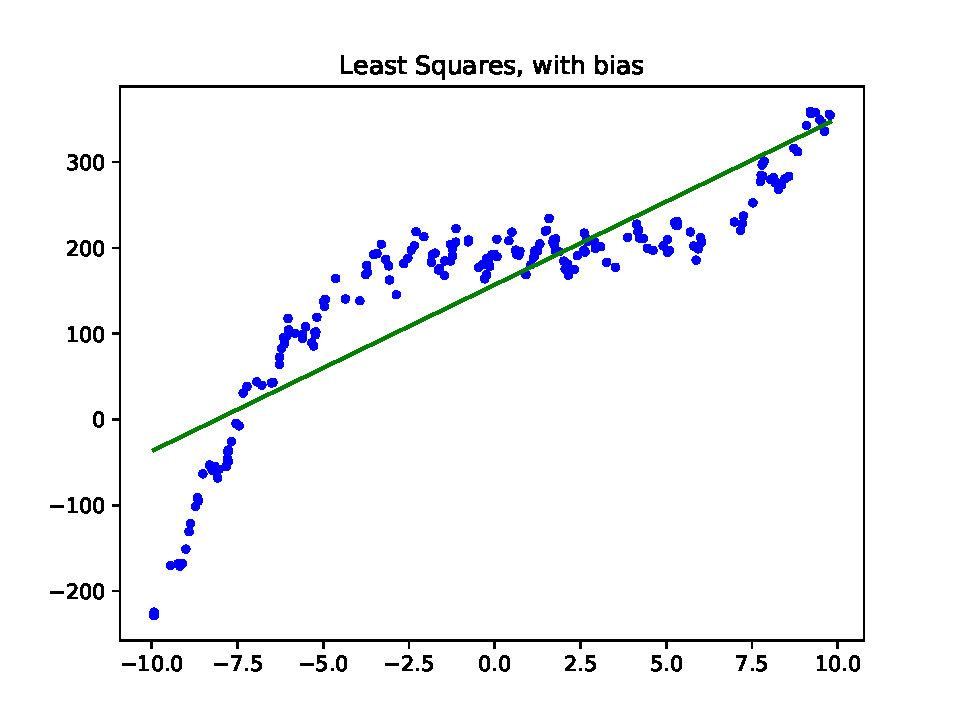
\includegraphics{../figs/least_squares_bias.pdf}
\\ New training error: 3551.3
\\ New test error: 3393.9

\subsection{Polynomial Basis}
\rubric{code:4,reasoning:1}

Adding a bias variable improves the prediction substantially, but the model is still problematic because the target seems to be a \emph{non-linear} function of the input.
Complete \emph{LeastSquarePoly} class, that takes a data vector $x$ (i.e., assuming we only have one feature) and the polynomial order $p$. The function should perform a least squares fit based on a matrix $Z$ where each of its rows contains the values $(x_{i})^j$ for $j=0$ up to $p$. E.g., \emph{LeastSquaresPoly.fit(x,y)}  with $p = 3$ should form the matrix
\[
Z =
\left[\begin{array}{cccc}
1 & x_1 & (x_1)^2 & (x_1)^3\\
1 & x_2 & (x_2)^2 & (x_2)^3\\
\vdots\\
1 & x_n & (x_n)^2 & (x_N)^3\\
\end{array}
\right],
\]
and fit a least squares model based on it.
\blu{Hand in the new class, and report the training and test error for $p = 0$ through $p= 10$. Explain the effect of $p$ on the training error and on the test error.}

Code can be found in $code/linear\_model.py$. \\\\
p=0 \\
training error:15480.5 \\
test error:14390.8 \\\\
p=1 \\
training error:15480.5 \\
test error:14390.8 \\\\
p=2 \\
training error: 3551.3 \\
test error: 3393.9 \\\\
p=3 \\
training error:2168.0\\
test error:2480.7\\\\
p=4\\
training error:252.0\\
test error:242.8\\\\
p=5\\
training error: 251.5\\
test error:242.1\\\\
p=6\\
training error:251.1\\
test error:239.5\\\\
p=7\\
training error:248.6\\
test error:246.0\\\\
p=8\\
training error:247.0\\
test error: 242.9\\\\
p=9\\
training error: 241.3\\
test error:246.0\\\\
p=10\\
training error:235.8\\
test error:259.3\\\\

As p increases, the model becomes more “complex” because it can reach more specific values with higher polynomials so it fits the data more appropriately. This is why both training and test error decrease as p increases. The test error spikes at p=10 because of overfitting of the data.

\section{Non-Parametric Bases and Cross-Validation}

Unfortunately, in practice we often don't know what basis to use.
However, if we have enough data then we can make up for this by using a basis that is flexible enough to
model any reasonable function. These may perform poorly if we don't have much data, but can
 perform almost as well as the optimal basis as the size of the dataset grows.
Using the same data set as in the previous question, 
in this question you will explore using Gaussian radial basis functions (RBFs),
 which have this property. These RBFs depend on a hyperparameter $\sigma$, which
 (like $p$ in the polynomial basis) can be chosen using a validation set.
 In this question, you will also see how cross-validation allows you to tune
 parameters of the model on a larger dataset than a strict training/validation split would allow.


\subsection{Proper Training and Validation Sets}
\rubric{reasoning:3}

If you run \verb|python main.py -q 4|, it will load the dataset and split the training examples
 into ``train'' and ``validation'' sets. It will then search for the best value of $\sigma$
 for the RBF basis.\footnote{if you look at the code you'll see that it also uses a tiny bit of regularization since $Z^TZ$ tends to be very close to singular; more on this later in the course.}
  Once it has the ``best" value of $\sigma$, it re-trains on the entire dataset and reports the
  training error on the full training set as well as the error on the test set.

Unfortunately, there is a problem with the way this is done: the data isn't shuffled before being split.
As a result, the IID assumption is badly broken and we end up with poor test error. Here is the plot:

\centerfig{.7}{../figs/least_squares_rbf_bad.pdf}


\blu{Fix the problem by either randomizing the split yourself or using \texttt{sklearn.model\_selection.train\_test\_split} with \texttt{train\_size=0.5}. Compare the train/test errors and plot before vs. after fixing this problem.}

The training/test error is much smaller after the split compared to before the split. As you can see in the plot below, the fit is much more accurate. \\
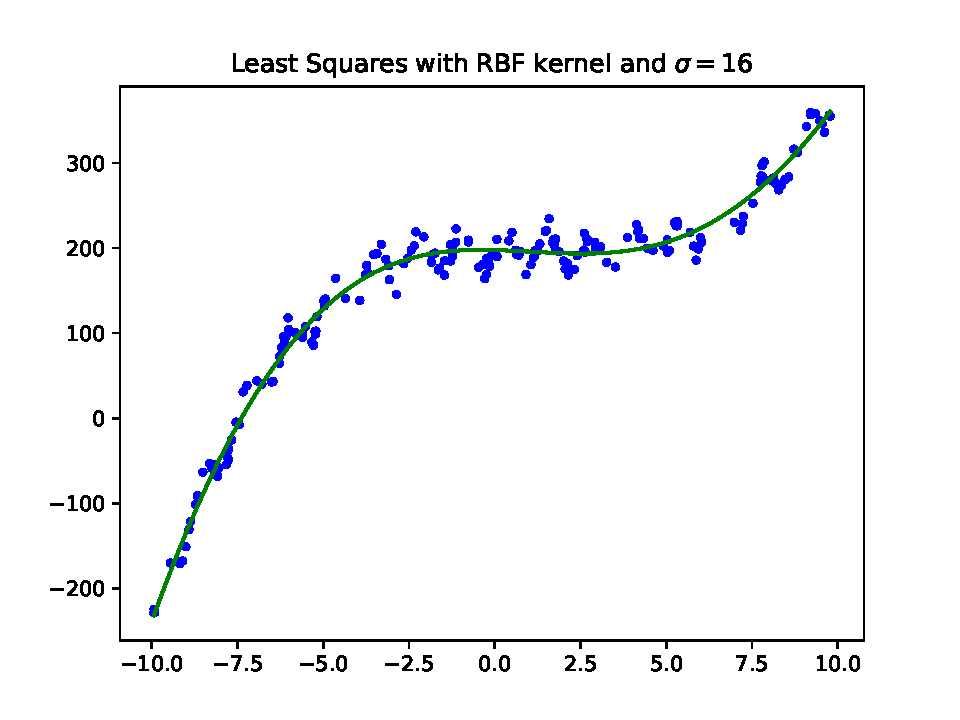
\includegraphics{../figs/least_squares_rbf_good.pdf}

\subsection{Cross-Validation}
\rubric{code:3,reasoning:1}

Now that we've dealt with the randomization, something's still a bit disturbing:
if you run the script more than once it might choose different values of $\sigma$.
This variability would be reduced if we
had a larger ``train'' and ``validation'' set, and one way to simulate this is
with \emph{cross-validation}. 

\enum{
\item What are two different ``best'' values of $\sigma$ you've observed after re-running the code a few times? (Not all students will have the same answer here; that's OK.) \\\\
16, and 8.
\item Implement 10-fold cross-validation to select $\sigma$, and hand in your code. What value of $\sigma$ does this procedure typically select? \\\\
Typically selects 1. The code can be found in $code/main.py$.
\\ 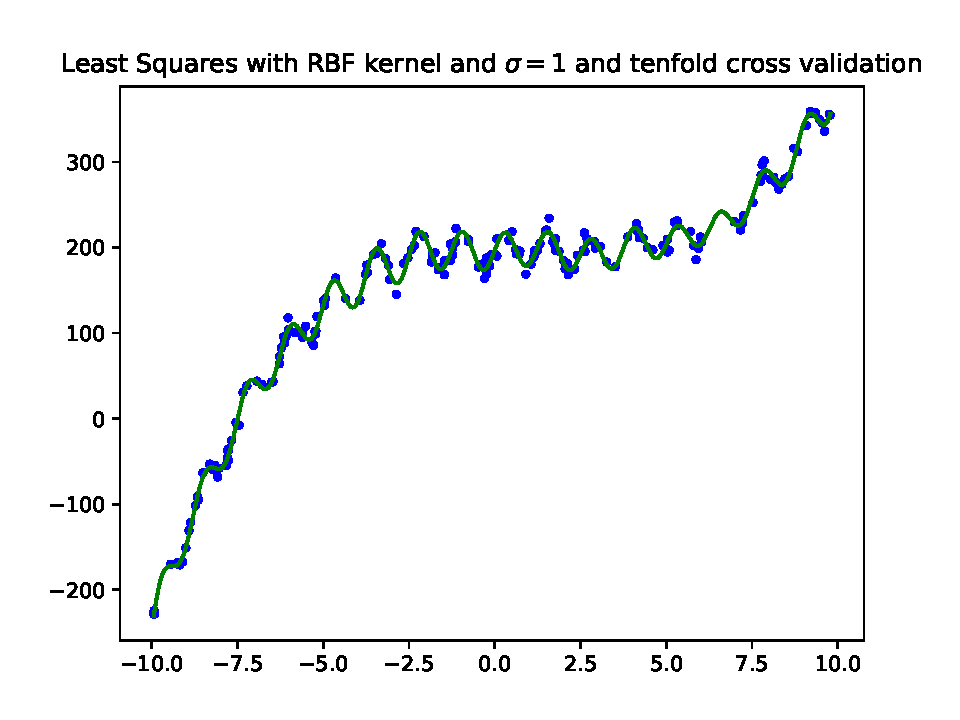
\includegraphics{../figs/least_squares_rbf_tenfold_cross_validation.pdf}
}


\subsection{Cost of Non-Parametric Bases}
\rubric{reasoning:3}

When dealing with larger datasets, an important issue is the dependence of the
computational cost on the number of training examples $n$ and the number of
features $d$. \blu{What is the cost in big-O notation of training the model
on $n$ training examples with $d$ features under (a) the linear basis and
(b) Gaussian RBFs (for a fixed $\sigma$)? What is the cost of
classifying $t$ new examples under each of these two bases? When are RBFs
cheaper to train? When are RBFs cheaper to test?}

The cost of training a model on $n$ training examples using linear basis is: $O(nd^2 + d^3)$. \\
The cost of training a model on $n$ training examples using RBFs is: $O(n^2d + n^3)$. \\
The cost of classifying $t$ new test examples using linear basis is: $O(td)$. \\
The cost of classifying $t$ new test examples using RBFs is: $O(tnd)$. \\
RBFs are cheaper when $d$ is much bigger than $n$ for training. \\
RBFs are never cheaper to test.

\section{Very-Short Answer Questions}

\subsection{Essentials}
\rubric{reasoning:10}

\enum{
\item In regression, why do we compute the squared error $(y_i - \hat{y}_i)^2$ rather than testing the equality $(y_i = \hat{y}_i)$? \\\\
Any graph that uses continuous values should used squared distances, rather than absolute distances because it gives the loss a proper range rather than just a very specific value.
\item Describe a situation in which the least squares estimate would not be unique when $d=2$ and $n=4$. \\\\
When all the n are in the same co-ordinate - when both features yield the exact same result.
\item What is the computational complexity of computing the closed-form (exact) solution to a linear least squares problem where we have one feature ($d = 1$) and use polynomial basis of degree $p$? \\\\
$O(nd^2 + d^3):$
$nd^2$ = the cost of creating a new matrix and $d^3$ = the cost of solving the linear system
\item In what circumstance would a regression tree with linear regressions at the leaves be a better choice
than a linear least squares regression model? \\\\
A combination of linear functions, a piecewise looking function
\item When fitting a model, why do we care if our loss function is convex?\\\\
Because in convex functions, the local minimum is also the global minimum.
\item When should we consider using gradient descent to approximate the solution to the least squares problem instead of exactly solving it with the closed form solution?\\\\
Not all problems have a closed form solution. Also, gradient descent can have a lower complexity depending on the number of iterations required, vs. closed form which always requires $O(nd^2 + d^3)$
\item Why is optimization non-trivial? Can't we just set the gradient to zero and be done immediately?\\\\
Not every problem has a closed form solution, and the minimum isn't always exactly 0. Plus, setting the gradient to 0 can cause the model to overfit.
\item Why do we need gradient descent for the robust regression problem, as opposed to just using the normal equations? Hint: it is NOT because of the non-differentiability. Recall that we used gradient descent even after smoothing away the non-differentiable part of the loss.\\\\
Not squaring the distances gives us a robust regression because big distances aren't amplified.
\item What is the problem with having too small of a learning rate in gradient descent?\\\\
We will need too many iterations to converge to the optimal solution.
\item What is the problem with having too large of a learning rate in gradient descent?\\\\
We will skip the optimal solution.
}

\end{document}
